\documentclass{ctexart}

\usepackage[backend=biber, style=numeric, sorting=ynt]{biblatex}
\addbibresource{refs.bib}

\usepackage{bm}
\usepackage{amsmath}
\usepackage{lmodern}
\usepackage{graphicx}
\usepackage{indentfirst}

\title{针对密集物体检测的焦点损失}
\date{2018 \\ February}
\author{Tsung-Yi Lin, Priya Goyal, Ross Girshick, Kaiming He, Piotr Dollar
\and Facebook AI Research (FAIR)}
\begin{document}
\maketitle
\begin{figure}[h] \label{fig:focal_loss}
    \centering
    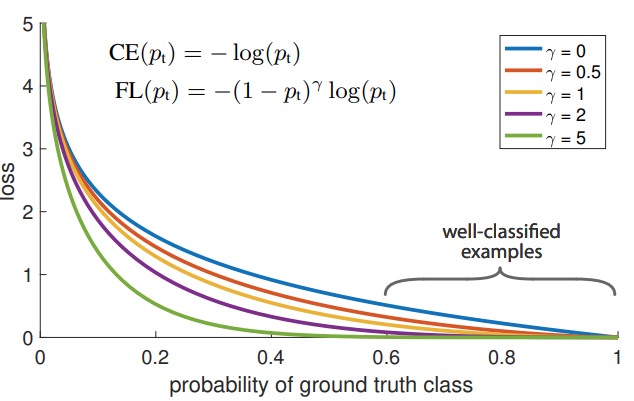
\includegraphics[width=.8\textwidth]{images/focal_loss.png}
    \caption{我们提出了一个名为焦点误差的损失,它在标准的交叉熵损失上加入了一个$(1-p_t)^\gamma$因子。设置$\gamma > 0$将会减少对于分类良好($p_t > .5$)例子的相对损失,从而更加专注于难的、错误分类的例子。正如我们的实验将要阐明的,我们提出的焦点误差使得在存在大量简单背景例子的情况下可以训练得到高精度密集物体检测器。}
\end{figure}
\begin{abstract}
    目前精度最高的检测器是由R-CNN普及、基于双阶段方法的,其中一个分类器被应用在一系列稀疏的候选物体位置上。与之相较的是,在物体可能位置的常规密集采样的单阶段检测器有更快和更简便的潜能,但是与双阶段的检测器精度相差较远。在这篇文章中,我们调研了这种情况的原因。我们发现在训练密集检测器过程中遇到的前景背景类别的极度不平衡是重要原因。我们通过重塑标准的交叉熵损失,降低分类良好的实例的损失的权重来解决这个类别不平衡问题。我们的焦点损失专注于在一系列稀疏的难例上训练,并防止了大量简单的负例在训练过程中压倒检测器。为了评估我们的损失的有效性,我们设计并训练了一个我们起名为RetinaNet的密集检测器。结果显示,当我们使用焦点损失训练时,RetinaNet可以匹配单阶段检测器的速度同时超过所有现有两阶段检测器的精度。
\end{abstract}
\section{introduction}
现有的sota物体检测器是基于两阶段的候选区域驱动机制的。正如R-CNN\cite{r_cnn}框架中所普及的,第一个阶段生成稀疏的候选物体位置,第二阶段使用卷积神经网络将每一个候选位置分类为某一种前景或者背景。通过一系列的改进,双阶段框架始终在COCO基准数据集\cite{coco}上达到高准确度。\par
尽管双阶段检测器获得了成功,但是一个自然的问题是:简单的单阶段检测器可以达到相似的准确率吗?单阶段检测器被应用在物体位置、尺寸和长宽比的普通的密集采样上。近期单阶段检测器的工作,例如YOLO\cite{yolo, yolov2}和SSD\cite{ssd},展示了光明的结果,得到了精度为sota双阶段检测器10\%到40\%的更快速的检测器。\par
这篇文章更进一步推动了信封:开创性地,我们提出了一个可以匹配更加复杂的双阶段检测器例如特征金字塔网络(FPN)\cite{fpn}或者Faster R-CNN\cite{faster_r_cnn}的变种Mask R-CNN\cite{mask_r_cnn},的最好COCO平均精度的单阶段检测器。为了达到这一结果,我们将训练过程中的类别不平衡视为阻碍单阶段检测器达到sota准确率的主要障碍,并提出了一个新的损失函数来消除这一障碍。\par
类似R-CNN的检测器通过两阶段级联和启发式采样来类别不平衡问题。候选阶段快速减少了候选物体位置的数量至一个较少的数量(例如1-2k),过滤掉了大部分背景采样。在第二个分类阶段,通过启发式采样,例如固定的前景背景比例(1:3),或者在线难例挖掘来维持前景和背景间的可管理平衡。\par
与之对比的是,一阶段检测器要出了在图片上规律采样得到的更多的候选物体位置。在实践中,我通常相当于枚举大约10万个位置,这些位置密集地覆盖了空间位置、尺寸和长宽比。虽然可以使用类似的启发式采样,但是由于训练过程仍然被轻易分类的背景例子统治,所以它仍然是无效的。这种无效是物体检测中的经典问题,通常通过例如bootstrapping或者难例挖掘来解决。\par
在这篇文章中,我们提出了一个新的损失函数,相较于以前方法,它是解决类别不平衡问题的更加有效的替代品。如图\ref{fig:focal_loss}所示,这个损失函数是动态缩放的交叉熵损失,缩放因子随着正确类别的置信度上升而衰减至0。直觉上,这个缩放因子可以在训练中自动降低简单例子的贡献并快速让模型将注意力集中在难例。实验显示,我们提出的焦点损失使得我们可以训练一个显著优于其他通过启发性采样或者难例挖掘训练得到的高精度的单阶段检测器。最后,我们发现焦点损失的具体形式并不关键,我们展示了其他的形式也可以达到类似的效果。\par
为了阐明我们提出的焦点损失的有效性,我们设计了一个简单的名为RetinaNet的单阶段物体检测器,因其在输入图片中对物体位置的密集采样而得名。它的设计具有高效的网络中特征金字塔以及锚框的使用。它从[]中借鉴了一系列近期的想法。RetinaNet既高效又准确。如图二所示,我们最好的模型,基于ResNet-101-FPN主干网络,在COCO上达到了39.1的平均精度同时达到了5fps的速度,超过了以前的包括单阶段和双阶段检测器的所有最好单模型结果。
\section{焦点损失}
设计焦点损失是为了解决单阶段检测器的训练过程中前景背景类别极度不平衡(例如1:1000)的问题。我们从二分类的交叉熵损失开始介绍焦点损失:
\begin{equation}
    CE(p, y)=\left\{
    \begin{aligned}
         & -\log(p)   & \text{if }y=1     \\
         & -\log(1-p) & \text{otherwise.}
    \end{aligned}
    \right.
\end{equation}
上述$y\in \{ \pm 1 \}$表示真实类别,$P \in [0,1]$是模型模型估计的标签为$y=1$的类别的概率。出于符号上的简便,我们定义$p_t$:
\begin{equation}
    p_t = \left\{
    \begin{aligned}
         & p     & \text{if }y=1     \\
         & 1 - p & \text{otherwise,}
    \end{aligned}
    \right.
\end{equation}
并重写$CE(p, y)=CE(p_t)=-\log(p_t)$。\par
交叉熵损失可以被视为图\ref{fig:focal_loss}中的顶部蓝色曲线。从图像中可以轻易看到,这个损失的一个显著特性是即使是轻松分类($p_t\gg .5$)的例子,也会产生不平凡的损失。当将大量简单例子的损失相加,这些较小的损失将会压倒稀少的类别。\par
\subsection{平衡的交叉熵}
解决类别不平衡的一种常见方法是为类别1引入加权因子$\alpha \in [0, 1]$,为类别-1引入$1-\alpha$。在实际中,$\alpha$可能被设置为类别频率的倒数或者被视为通过交叉验证设置的超参数。出于符号上的简便,我们使用类似定义$p_t$的方法定义$\alpha_t$。我们将$\alpha$平衡的交叉熵损失写为:
\begin{equation}
    CE(p_t)=-\alpha_t\log(p_t)
\end{equation}
这个损失是交叉熵损失的简易扩展,我们将它视为针对我们提出的焦点误差的实验基线。
\subsection{焦点损失的定义}
正如我们的实验将要展示的,训练密集检测器中遇到的大量类别不平衡压垮了交叉熵损失。可以轻易分类的负例组成了损失的主体并统治了梯度。虽然$\alpha$平衡了正负例的重要程度,但是它没有将难易例作区分。取而代之,为了降低简单例子的权重并因此集中注意在难负例上训练,我们提出变形损失函数。\par
更加正式的,我们提出通过可调整的注意力参数$\gamma \ge 0$为交叉熵损失添加调制因子$(1-p_t)^\gamma$。我们定义焦点损失为:
\begin{equation}
    FL(p_t)=-(1-p_t)^\gamma\log(p_t)
\end{equation}
在图\ref{fig:focal_loss}中,我们为$\gamma \in [0, 5]$中的不同值的焦点损失做了可视化。我们注意到了焦点损失的两个性质。1)当样本被错误分类同时$p_t$很小,此时调制因子接近1,因此损失没有被影响。当$p_t\rightarrow 1$,因此趋向于0因此分类良好的例子权重被降低。2)注意力参数$\gamma$平滑地调整简单例子权重减低的速率。当$\gamma=0$是,焦点损失和交叉熵损失等价,随着$\gamma$增加,调制因子的影响也增加(我们发现$\gamma=2$在我们的实验中效果最好)。\par
直觉上,调制因子减少了简单例子对于损失的贡献并扩展了例子在损失函数接收低损失的范围。例如,当$\gamma=2$时,一个被分类为$p_t=0.9$的例子比对应交叉熵的损失小100倍,$p_t\approx 0.968$的例子比对应交叉熵的损失小1000倍。这反过来会增加更正错误分类例子的重要性(当$\gamma = 2$时,对于$p_t \leq .5$的例子损失最多会缩小4倍)。\par
实际上我们使用了$\alpha$平衡版本的焦点误差:
\begin{equation}
    FL(p_t)=-\alpha_t(1-p_t)^\gamma\log(p_t).
\end{equation}
因为它相较于无$\alpha$平衡的版本有轻微的准确率提高,所以我们在实验中采用了这个形式。最后,我们注意到将计算$p$的sigmoid操作和计算损失结合起来的损失层实现会有更好的数值稳定性。\par
尽管我们在主要试验结果中使用了上述的焦点损失定义,但是它的准确形式并不关键。我们在附录中考虑了焦点损失的其他实例并阐明了它们同样有效。
\subsection{类别不平衡和模型初始化}
二分类模型被默认初始化为输出$y=-1$或$1$的概率相同。在这样的初始化下,由于类别不平衡,由于经常出现的类别产生的损失会统治最终的损失从而导致在早期训练的不稳定。为了解决这个问题,我们在\textit{训练的开始}为模型为稀有类别估计的概率$p$引入了“先验”的概念。我们记先验为$\pi$并通过设置使得模型对于稀有类别的预测$p$很低,例如0.01。我们注意到这是对模型初始化而不是损失函数的改变。我们发现这会在类别不平衡的情况下为交叉熵损失和焦点损失提高训练的稳定性。
\subsection{类别不平衡和两阶段检测器}
两阶段检测器通常通过交叉熵损失训练而不会使用$\alpha$平衡或者我们提出的损失。取而代之的是,它们通过两种机制来解决类别不平衡问题:1)两阶段级联和2)有偏向性的样本采样。第一个级联阶段是通过物体位置候选机制来将近乎无穷的可能物体位置减少至一到两千。重要的是,选择的候选位置并不是随机的,而很有可能对应于真实的物体位置,这移除了很大一部分的简单负例。当训练第二阶段时,通常通过有偏向性的采样来构造包含例如1:3的正负样本比的迷你批。这个比例就像是通过采样实现的隐式$\alpha$平衡因子。我们提出的焦点误差被设计通过损失函数直接解决单阶段检测系统中的这些问题。
\section{RetinaNet检测器}
RetinaNet是一个有主干网络和两个特定任务的子网络组成的单一统一网络。主干网络负责计算整个输入图片的卷积特征,是一个现成的卷积网络。第一个子网络负责在主干网络的输出上进行卷积物体分类;第二个网络则进行卷积边界框回归。正如图\ref{fig:network}所示,两个子网络设计简单,我们提出了特意针对单阶段密集检测。虽然这些组件的细节有很多可能的选择,但是大多数设计参数对于得到如实验部分所示的结果并不敏感。我们接下来介绍RetinaNet的每一个组成部分。\par
\begin{figure}[h] \label{fig:network}
    \centering
    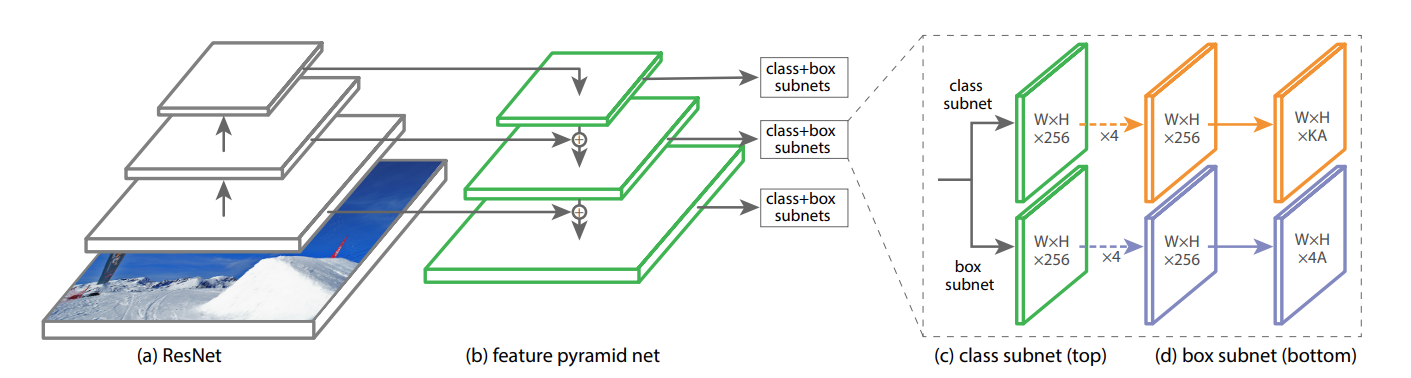
\includegraphics[width=.8\textwidth]{images/network.png}
    \caption{单阶段\textbf{RetinaNet}网络结构在ResNet架构上使用特征金字塔网络(FPN)\cite{fpn}主干网络(a)来生成一个丰富的多尺度卷积特征金字塔(b)。RetinaNet在主干网络上连接了两个子网络,一个用于为锚框分类(c),另一个则是为了从锚框回归到真实的物体框(d)。网络特意被设计的很简单,这使得这个网络可以专注于新颖的焦点误差函数,它在运行更快的基础上,消除了一阶段检测器和例如FPN基础上的Faster R-CNN等sota两阶段检测器间的精度差距。}
\end{figure}
\textbf{Feature Pyramid Network Backbone:} 我们借用\cite{fpn}中的特征金字塔网络来作为RetinaNet的主干网络。简单来说,如图\ref{fig:network}(a)-(b)所示,特征金字塔网络通过自上而下的通路和旁路连接来增强标准的卷及网络,这样网络可以高效地从一个单分辨率输入图片构建表意丰富的多尺度特征金字塔。金字塔的每一个层级可以被用来检测不同尺度的物体。正如它在RPN和DeepMsk-style区域候选所带来的提升和在例如Fast R-CNN和Mask R-CNN\cite{mask_r_cnn}等两阶段检测器所表明的,特征金字塔网络相较于全卷积网络提高了多尺度预测能力。\par
遵循\cite{fpn},我们在ResNet架构基础上构建了特征金字塔网络。我们通过$P_3$到$P_7$层级构建了一个金字塔,其中$l$表示金字塔层级(这里$P_l$的分辨率比输入低$2^l$)。正如\cite{fpn},所有的金字塔层级的通道数$C$均为256。金字塔的细节基本上遵循\cite{fpn},除了一些细小的不同。虽然一些设计选择并不关键,我们强调特征金字塔网络的使用是关键的;初步的实验仅使用最终的ResNet特征获得了更低的AP。\par
\textbf{Anchors:} 我们使用了具有变换不变性的锚盒,类似在RPN变种\cite{fpn}中的使用。锚的面积从金字塔层级$P_3$到$P_7$分别为$32^2$到$512^2$。和\cite{fpn}中相同,在每一个金字塔层级我们使用三个长宽比$\{ 1:2, 1:1, 2:1 \}$。为了相较于\cite{fpn}更加密集的尺度铺盖,我们在每一个层级添加了大小为原来三个长宽比锚的$\{ 2^0, 2^{1/3}, 2^{2/3} \}$的锚。这个设置提高了AP。每个层级总共有$A=9$个锚,关于网络的输入图像,跨越层级它们包含的尺度为$32-813$个像素点。\par
我们赋予每个锚一个长度为$K$的分类目标单热点向量,其中$K$是物体类别的数量,和一个长度为4的边界框回归目标向量。我们使用\cite{faster_r_cnn}中的分配策略,但是为了多类别检测做了修改,并调整了阈值。特别地,当锚和真实物体框的IoU高于0.5时,我们将锚分配给此真实物体框;如果它们的IoU为$[0, 0.4)$则分配给背景。由于每个锚最多被分配给一个物体框,所以我们将$K$标签向量中对应的值设置为1其他设置为0。如果某个锚没有被分配,也就是它的重叠区为$[0.4, 0.5)$,那么我们在训练中忽视它。框回归目标被作为锚和它对应的物体框的偏移,如果没有分配则忽视它。\par
\textbf{分类子网络:} 分类子网络预测物体出现在$A$个锚的空间位置的概率以及属于$K$个物体类别的概率。这个子网络是依附在每一个FPN层级的FCN,这个子网络的所有参数在所有的金字塔层级中共享。它的设计是简单的。对于给定的金字塔层级,对于通道数为$C$的输入特征图,子网络使用四个有$C$个卷积核并使用ReLU作为激活函数的$3 \times 3$的卷积层,并跟随一个有$K A$个卷积核的$3\times 3$卷积层。通过sigmoid来得到最终输出——也就是每一个空间位置的$K A$个二分类输出,如图\ref{fig:network}所示。在大部分实验中,我们使用$C=256$和$A=9$。\par
与\cite{faster_r_cnn}不同的是,我们的物体分类网络更深,并仅适用$3\times 3$卷积,并且没有与框回归共享子网络。我们发现这个更高层级的设计决定比超参数的具体值更加重要。\par
\textbf{框回归子网络:} 与物体分类子网络平行的是,我们为每个金字塔层级附加了一个更小的FCN来回归每一个锚和到附近的真实物体(如果存在的话)的偏移。框回归网络与分类网络的设计基本相同,除了它在每一个空间位置以$4A$个线性输出结束,如图\ref{fig:network}d所示。对于每个位置的$A$个锚,会有4个输出来预测锚和真实框的相对偏移(我们使用R-CNN中的标准框参数形式)。我们注意到不同于大部分的近期工作,我们使用了一个未知类别的边界框回归,它使用了更少的参数并同样有效。物体分类网络和框回归网络通过共同的结构,使用不同的参数。
\subsection{推理和训练}
\textbf{Inference:} RetinaNet形成了一个单独的由ResNet-FPN主干网络、一个分类子网络和一个框回归网络组成的FCN,见图\ref{fig:network}。如此,推理包含简单的前向传播。为了提高速度,在以0.05为阈值筛选后,在每一个FPN层级,我们最多使用前1000个高得分预测值来解码框预测值。为了得到最终的预测结果,来自所有层级的框将会合并并通过一个阈值为0.5的非最大抑制。\par
\textbf{焦点误差:} 我们在分类子网络上使用我们提出的焦点误差。正如我们将要展示的,我们发现使用$\gamma = 2$在实际中效果较好,同时RetinaNet对于$\gamma \in [0.5, 5]$鲁棒性较好。需要强调的是,当我们训练RetinaNet时,我们在所有每张图片的几乎十万个锚上使用焦点误差。这与为每一个批使用启发性采样(RPN)或者难例挖掘(OHEM,SSD)来选择一小部分锚(例如256)形成了对比。一张图片的总共焦点误差被计算为所有接近十万个锚的焦点误差之和,\textit{并通过被分配给真实框的锚的数量来归一化}。我们通过被分配锚的数量而不是总共锚的数量来归一化,是因为大部分锚是简单负例,在焦点误差上得到可以忽略的损失值。最后我们注意到$\alpha$,也就是分配给稀少类别的权重,也有一个稳定区间,当时它与$\gamma$相互作用使得有必要将二者一起选择(见表1a和1b)。大体上,$\alpha$应该随着$\gamma$增加而轻微减低(对于$\gamma=2$,$\alpha=0.25$效果最佳)。\par
\textbf{初始化:} 我们使用ResNet-50-FPN和ResNet-101-FPN作为主干网络进行实验。ResNet-50和ResNet-101模型在ImageNet1K上进行了预训练。我们使用了\cite{resnet}发布的模型。对于FPN新加入的层通过\cite{fpn}初始化。除了子网络中的最后,所有的新卷基层通过误差$b=0$和一个$\sigma=0.01$的高斯权重。对于分类子网络的最终卷基层,我们将偏差值设置为$b=-\log((1-\pi)/\pi)$,其中$\pi$表示在训练的开始阶段,所有的锚应该被标记标记为置信度为$~\pi$的前景。我们在实验中使用$\pi=.01$,但是结果对于特定的值有鲁棒性。正如在section above中解释的,这种初始化防止在训练的最初迭代中大量的背景锚生成大的、不稳定的损失。\par
\textbf{优化:} 我们使用随机梯度下降来训练RetinaNet。我们在8张GPU上使用批大小为16的同步随机梯度下降(每张GPU有2张图片)。除了特别指出的,所有模型都训练了90k个迭代,学习率初始为0.01,并在60k和80k此迭代时分别除10。除了特别指出,我们使用水平图像翻转作为唯一的数据增强。我们使用了0.0001的参数衰减和0.9的动量。训练损失函数是焦点损失和对于框回归的标准光滑$L_1$损失的和。模型训练时间从10小时到35小时不等。

\printbibliography

\end{document}